\section{Introduction to Neural Networks}
Neural Networks are a specific branch of the Artificial Intelligence (\emph{AI}) domain in computer science.
They get their inspiration from the fact that humans are able to fulfill complex tasks; hence, by replicating the low-level mechanisms of the human brain on computing systems, one can potentially construct high level algorithms with similar capabilities.

\subsection{The human brain}
Neglecting any functional description, the human brain can be described as an organ composed by neuron, glial cells, neural stem cells and blood vessels (Figure~\ref{fig:humanbrain}).
\begin{figure}[h]
    \centering
    \begin{subfigure}[b]{0.35\textwidth}
    \centering
    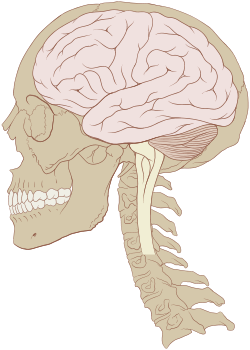
\includegraphics[width=0.4\textwidth]{images/humanbrain.png}
    \caption{A pictorial view of the human brain (from Wikipedia).}
    \label{fig:humanbrain}
    \end{subfigure}
    \hfill
        \begin{subfigure}[b]{0.55\textwidth}
        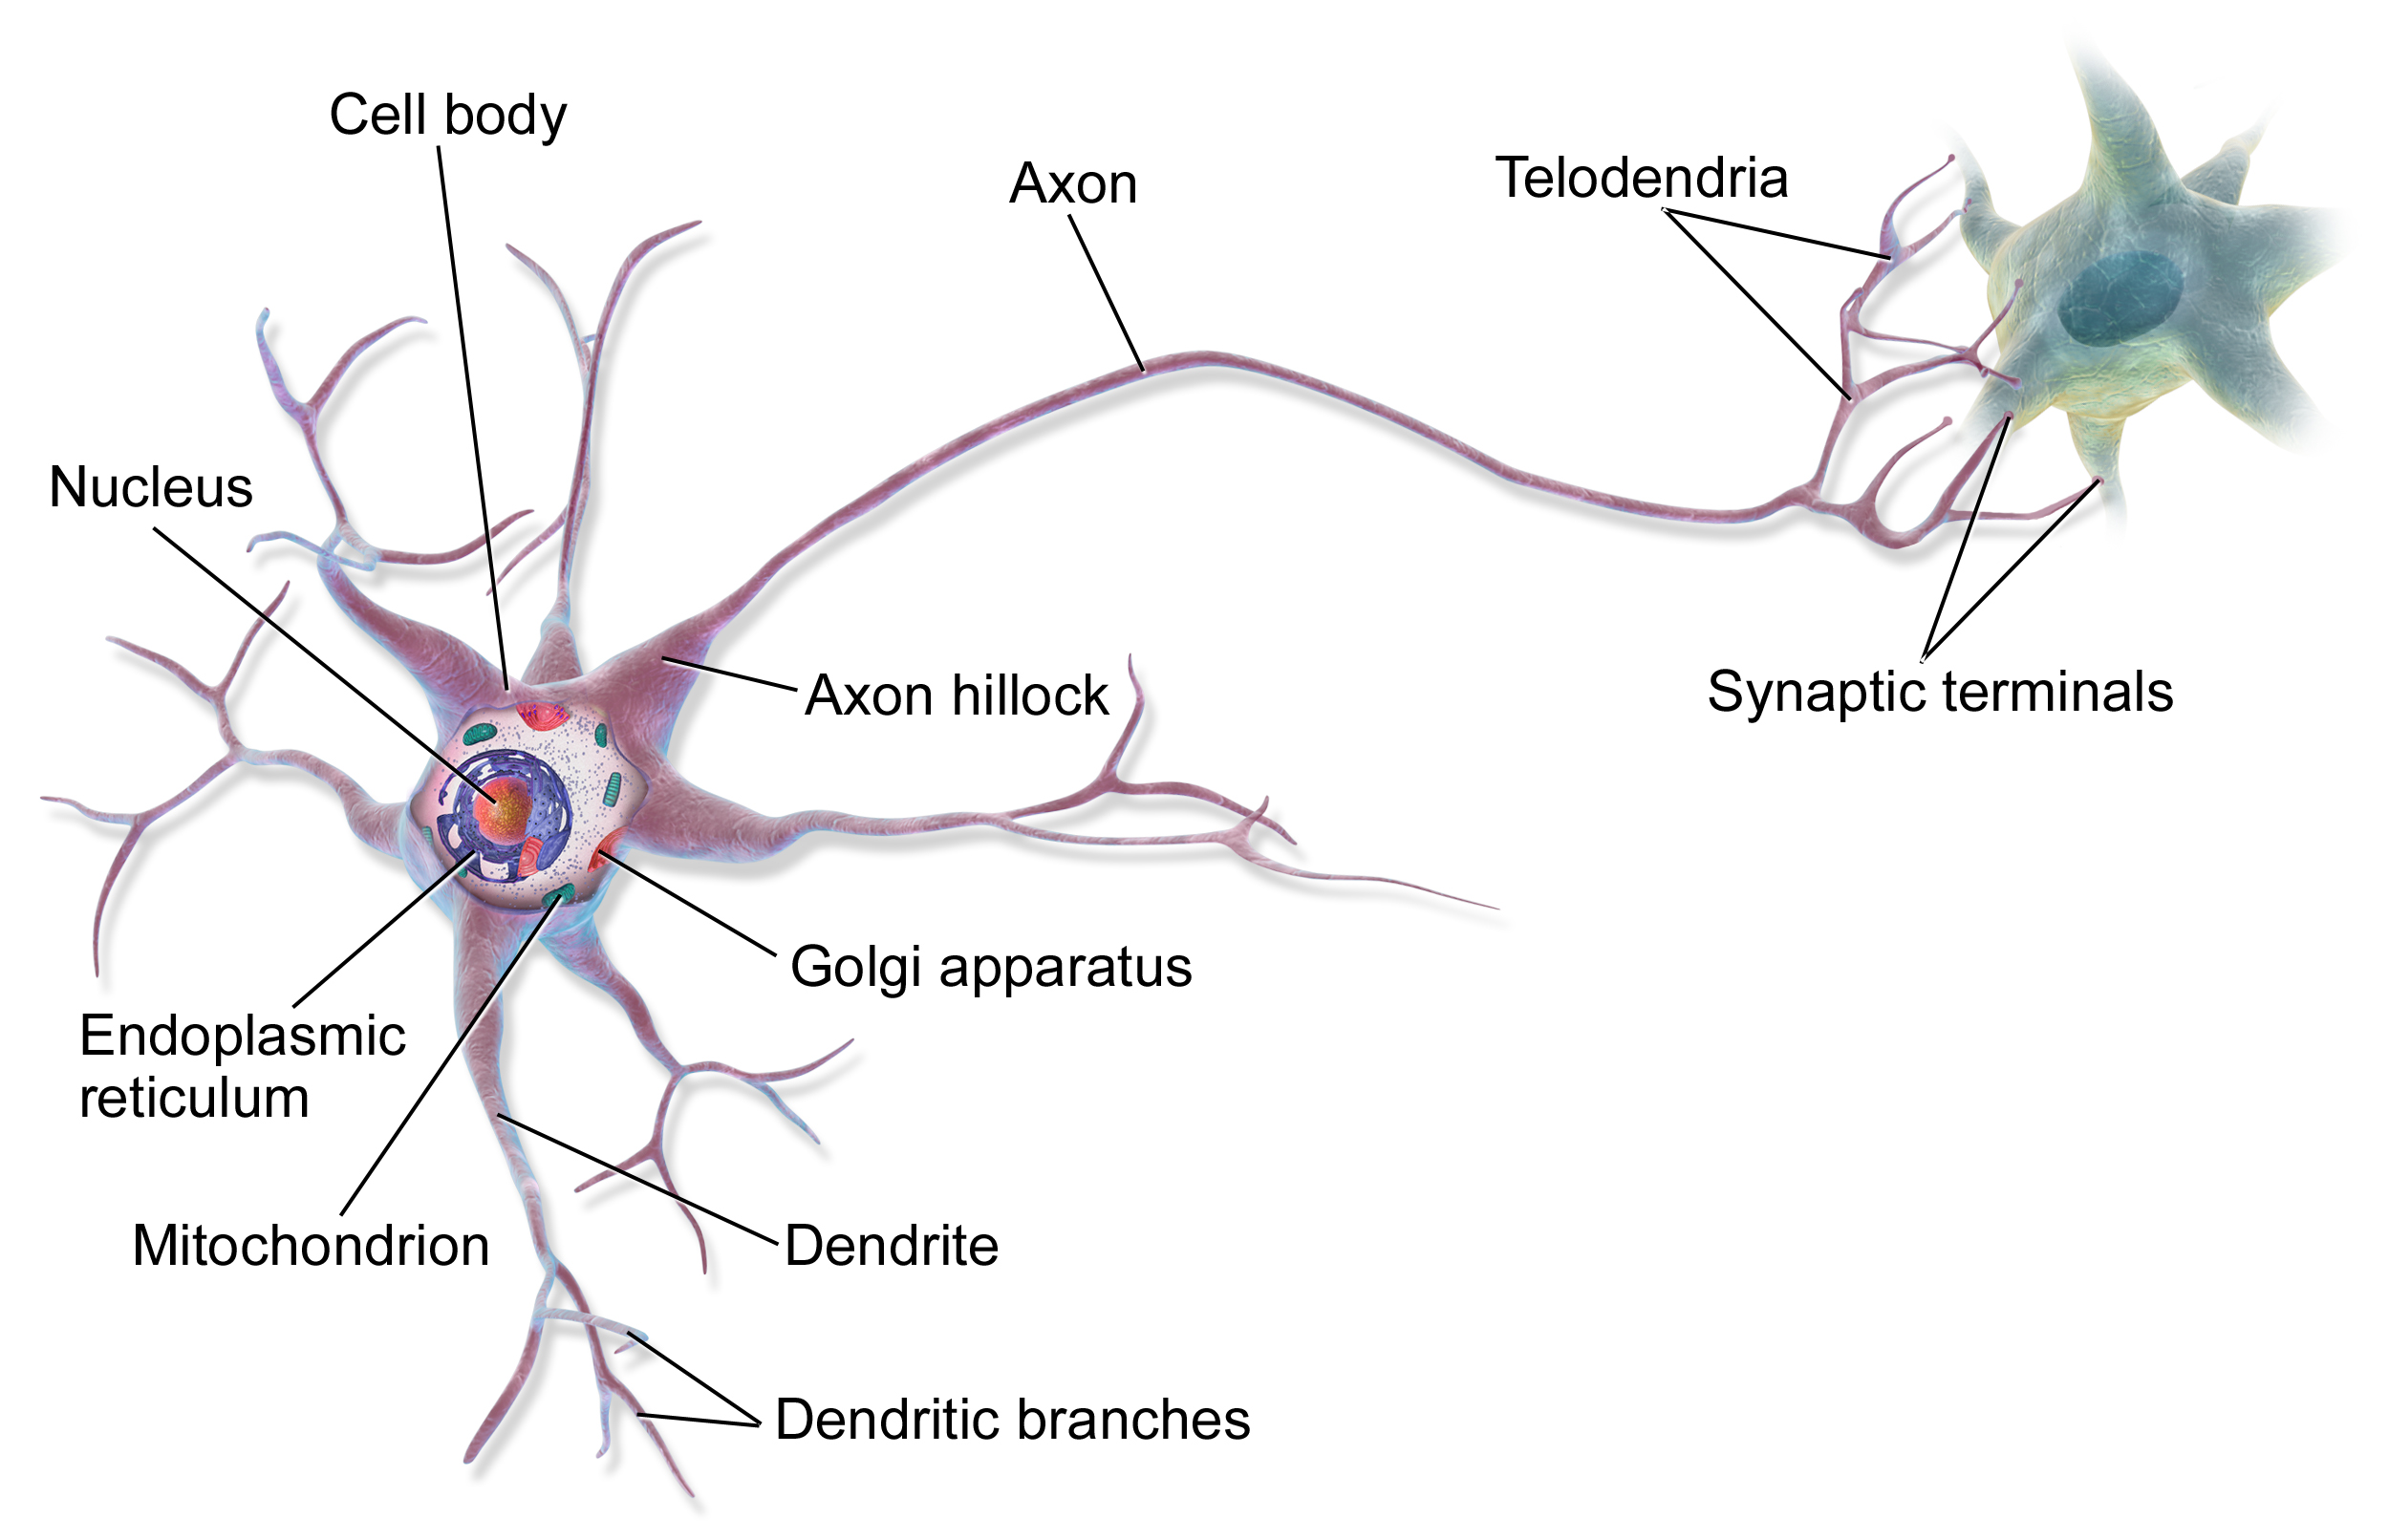
\includegraphics[width=0.8\textwidth]{images/Blausen_0657_MultipolarNeuron.png}
     \caption{The artificial neuron.}
     \label{fig:neuron}
        \end{subfigure}

\end{figure}
 With our current understanding, the neurons are the units performing basic "operations" within the human brain, and their aggregate response is generating the high-level behaviour typical of humans.
 A neuron, as sketched in Figure~\ref{fig:neuron}, is composed of three main units: a number of dendrites, the soma (the cell body), and an axion; the total size largely varies between different types of neurons; the neurons used for cognitive functions (as those in the grey matter of the brain) are usually short, XX $\mu$m.
Functionally, a neuron is able to generate an electric response on the axion (\emph{output}), depending on the electrical potential present at the synapses (\emph{inputs}) present on the dendrites, generating a quite low-level response mechanism. Neurons are \emph{chained} by connections between axions and dendrites, generating a mesh in which N neurons are connected via M synapses.
 The high-level response of the human brain to stimula is understood to come from the complexity of such mesh, with a standard human brain featuring $~10^{11}$ neurons each with $~7000$ synapses, for a total of $~10^{15}$ "connections".

 In literature various models of the neuron behavior have been proposed~\cite{neuronbe1, neuronbe2, neuronbe3}, %https://en.wikipedia.org/wiki/Biological_neuron_model
 here we will focus on the simplest yet most simple to implement in computer systems~\cite{artificialneuron} (see Figure~\ref{fig:artificialneuron}): %https://en.wikipedia.org/wiki/Artificial_neuron
 
 \begin{figure}[h]
    \centering
    \hfill
        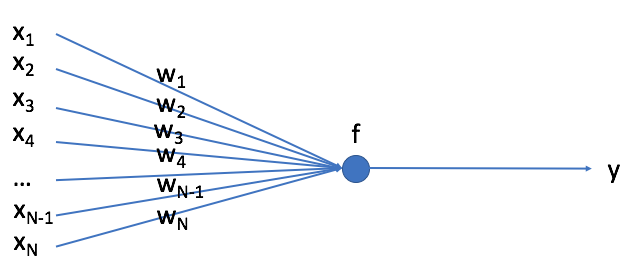
\includegraphics[width=0.9\textwidth]{images/artificialneuron.png}
     \caption{The artificial neuron.}
     \label{fig:artificialneuron}

\end{figure}
 
 in this model, the \emph{output} $y$ signal at the axion is assumed to be a function of the \emph{inputs} $x_i$ via
 \begin{equation}
   y = f(\sum_{i=1}^{N} w_i x_i)
   \label{eq:artificialneuron}
 \end{equation}
where $w_i$ are weights defined by chemical potentials at the synapses, and the function $f$ wants to model the non linearity of response of biological neurons with the \emph{inputs}; on top of this, the function $f$ is needed in the mathematical model in order to allow the description of non linear phenomena~\cite{nonlinearitytheorem}. The percepton~\cite{perceptron}, one of the first models used in literature for Neural Networks, uses a very similar model, with a simplified $f$ function which is simply
\begin{equation}
  f(\vec{x})= \begin{cases}
                1 &  \text{if}\  \sum_{i=1}^{N} w_i x_i >0 \\
                0 &  \text{otherwise}
              \end{cases}
\end{equation}
Today, two small modifications are typical when using Neural Networks:
\begin{itemize}
\item the addition of a further synapse $x_0$ which is always 1, as a bias to the system; its weight is referred to as $x_0$ or $b$ () as in \emph{bias}.
\item the use of continuous $f$ non linear functions, as the logistic~\cite{logistic} or the hyperbolic~\cite{hyperbolic} functions.
\end{itemize}

Neural networks are obtained by combining multiple neurons in \emph{networks}, usually in a layered structure: one layer is used to map the inputs, a few/many layers are \emph{hidden}, and a single layer used to to map the outputs. On top of that, more complex neurons an be used, for example including a "memory" cell, or presenting a recurrent behavior by reusing its output as one of the inputs. A full description of all the type of neurons and networks is beyond the scope of this chapter; in the following, the ones most relevant to Monte Carlo simulations will be presented wit more detail. For reference, still, a complete classification of currently relevant neural networks is shown in Figure~\ref{fig:types}.
\begin{figure}[h]
    \centering
    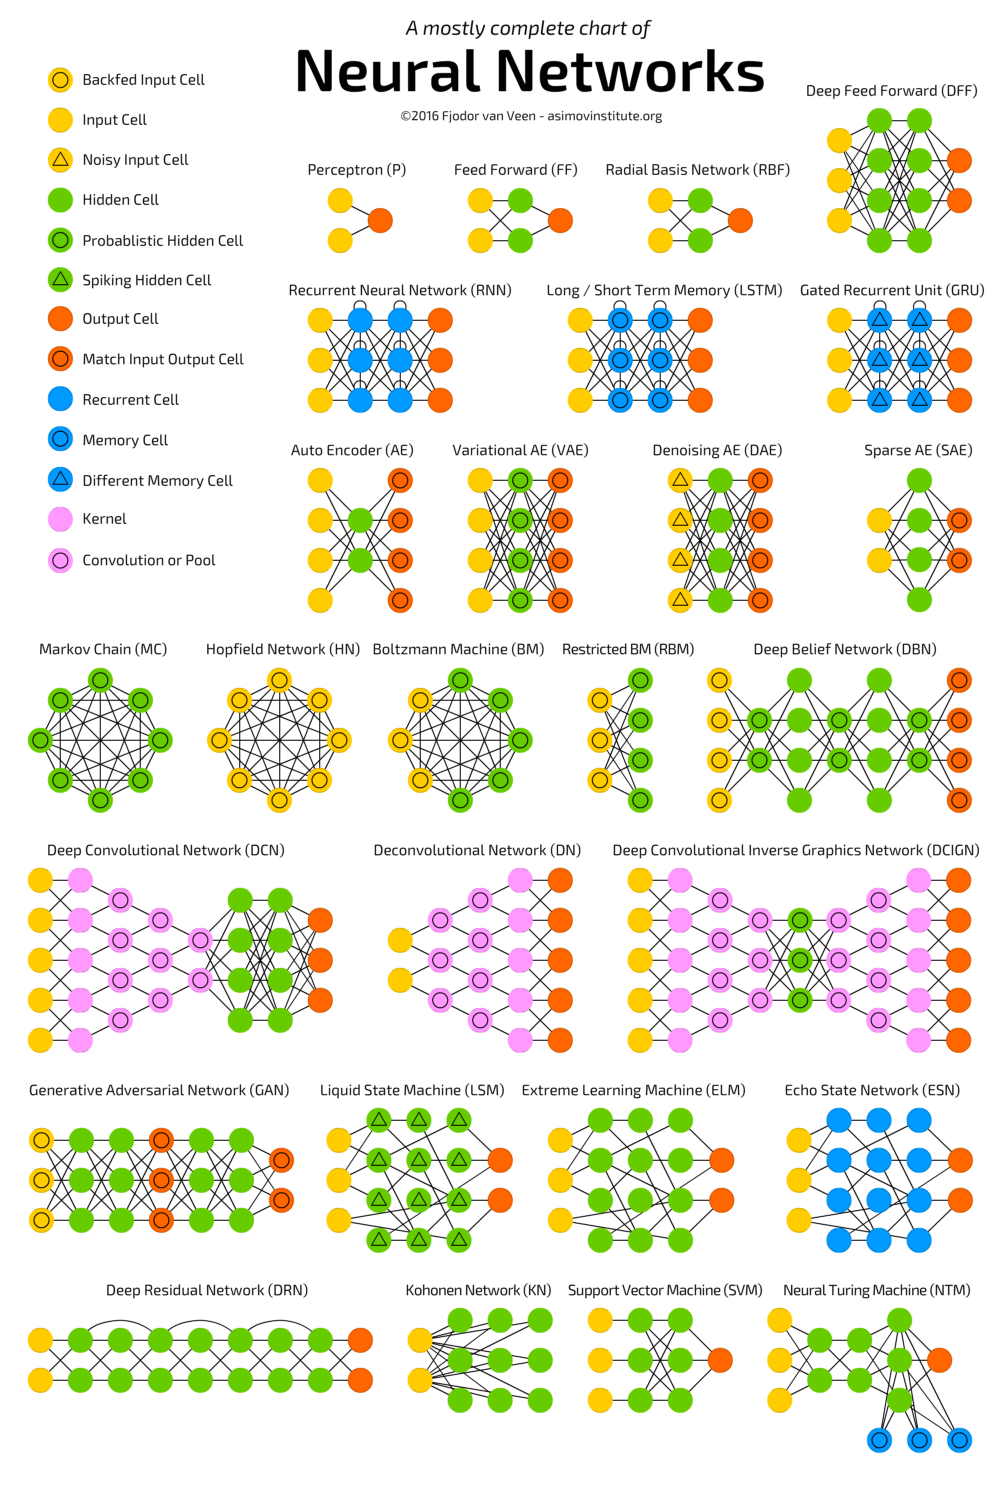
\includegraphics[width=0.9\textwidth]{images/types.png}
    \caption{Types of neurons and neural networks currently relevant in literature (Copyright F. van Veen 2016).}
    \label{fig:types}
\end{figure}
As clearly visible in the figure, some network topologies have an high number of hidden layers. While the Universal Approximation Theorem~\cite{nonlinearitytheorem} states that under quite generic conditions, a single hidden layer between inputs and outputs should be enough in all cases, networks used in science during the last decade tend to be "deep" (i.e. with many hidden layers). This has multiple motivations: on one side, the theorem states that it is possible to have just one hidden layers, but does not state with how many neurons (and it tends to be a very large number); on the other side, a deep structure tend to be better human readable, with cascade sub networks with a more identifiable and logical role. Hence, relevant networks in today's science tend to be deep.

The typical utilization pattern for a majority of network topologies is to feed them as input a large set of data representing the problem of interest, be it a medical image, a set of features or any output from the instrumentation, and at the same time provide the "expected output" from a so-called training set. The network adjusts its internal free degrees of freedom (the weights $w_i^j$ in equation~\ref{eq:artificialneuron}, extended to the $j$ neurons in the various layers) to better reproduce the desired answers, via minimization procedures which can be either numerical or analytical.

What has just been described is the training process for \emph{supervised} Neural networks, which rely on an externally provided "truth" to adjust for optimal performance, without having any a-priori knowledge of the physical process they want to reproduce.
Other topologies describe instead the \emph{unsupervised} Neural Networks, in which the training process just implies the utilization of datasets without the need to provide the correct answers". Examples of such networks will be provided in Section~\ref{sec:unsupervised}.


\subsection{Convolutional networks}
Convolutional networks are a useful subset of neural networks, which exhibit peculiar characteristics of being space invariant with respect of the inputs.

They are particularly interesting in the realm of Monte Carlo simulations, since the space invariance is a valuable characteristics: for example, a shower from an hadronic particle into a material, when far from the edges, does not depend on the specific entry point

\subsection{Recurrent networks}

\subsection{Generative Models}
The networks popular up to 10 years ago were mostly useful during a decision process, such has categorizing inputs (signal vs background, for example) or counting and defining specific regions inside it (segmentation, counting of lesions, etc).

In order to be applied to Monte Carlo simulations, instead, the capability to produce ("generate") an output as close as possible to reality, or to a more standard algorithm. In order to do this, different network topologies and strategies for training are relevant.

%It needs to be highlighted that none of the methods described in this chapter have any intrinsic knowledge of the physics involved in the simulation processes. They are "trained" on external data, which needs to be accurate as possible. While to some extent it is possible to think of a training process using data, in practice the data samples and setups to ensure a generic training is huge, and not easy to obtain in practice. Hence, standard training samples are usually provided via "old school" detailed simulation toolkits, like Geant4~\cite{g4} or FLUKA~\cite{fluka}; it is important to notice that the advent of Machine Learning techniques for Monte Carlo simulations does not imply that the latter will be less needed, on the contrary it will remain fundamental to have  understood and well tuned reference tools to be used to train AI inspired tools.

\subsubsection{Auto-Encoders and Variational Auto-Encoders}
\label{sec:unsupervised}
The autoencoders are a family of unsupervised Neural Networks designed to learn a lower dimensional representation (say N dimensions) out of a set of data (with M dimensions, M \textgreater N). The N dimension representation ("latent space") can be seen as coming from a a 

The easiest form of autoencoder is one in which the number of inputs and outputs equals to M, and where there is a layer at dimensionality N. The training is obtained by forcing the network to reproduce as close a possible the input features at the output layer, thus requesting the N-dimension space to be as sufficient as possible to represent the M-dimension inputs (see Figure~\ref{fig:autoencoder}).

\begin{figure}[h]
     \centering
     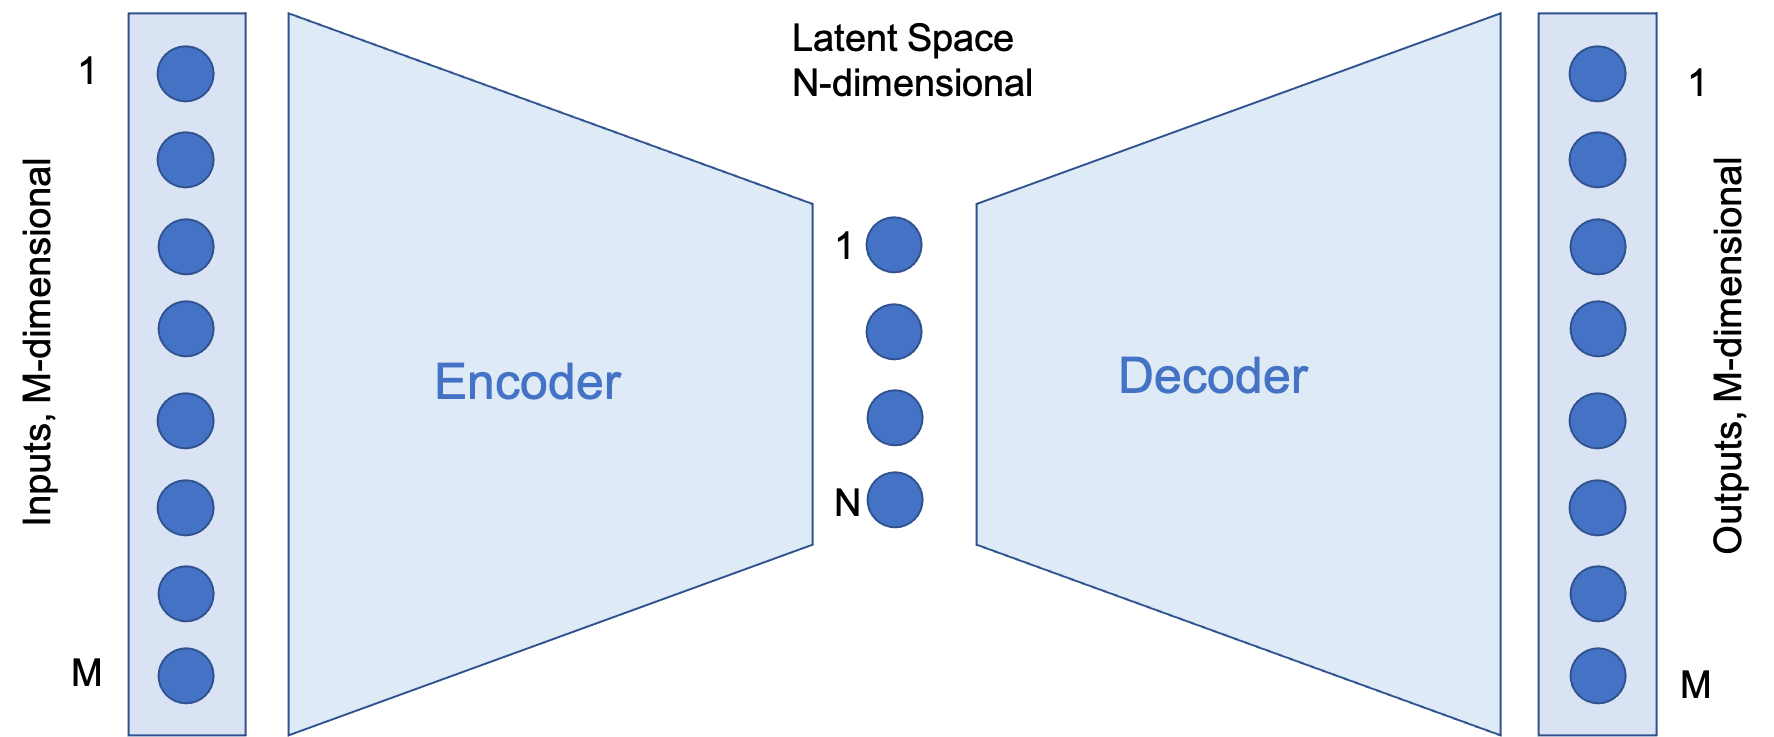
\includegraphics[width=0.85\textwidth]{images/autoencoder.png}
     \caption{An autoencoder in its simplest form.}
     \label{fig:autoencoder}
 \end{figure}
 
 Autoencoders in such form are used for two distinct purposes:
 \begin{itemize}
     \item auto-discover in the inputs hidden symmetries or underlying correlations, which can be used, for example, in lossy compression scheme or to drive understanding on the inputs themselves;
     \item since the network is trained on a specific data sample, it will minimize the difference outputs vs inputs on that specific dateaset. Once the same network is presented with 
 \end{itemize}
 

\subsubsection{Generative Adversarial Networks}
\subsubsection{Graph Networks}




